\section{Results}

Here, one can display figures, such as in \Cref{fig:example}.

\begin{figure}
    \centering
    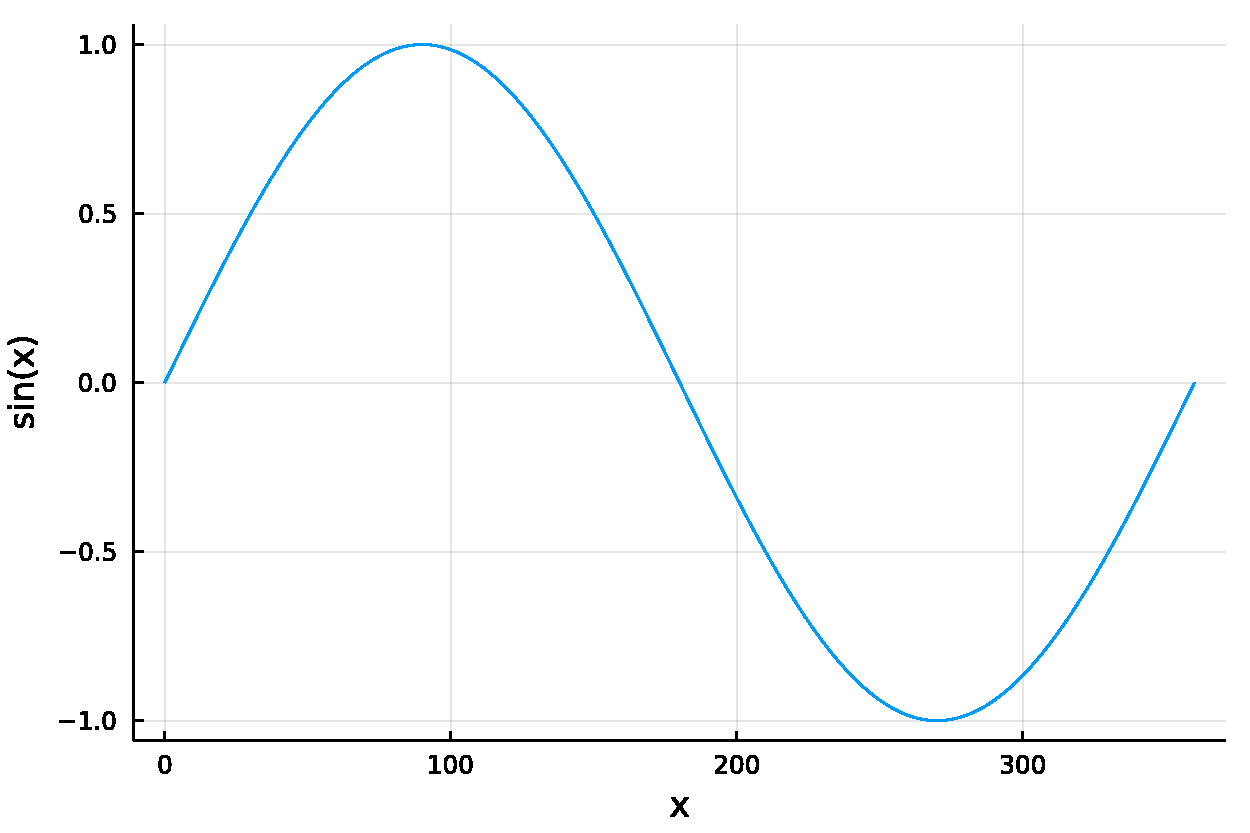
\includegraphics[width=\singlefigure]{figures/example.pdf}
    \caption{\label{fig:example} Shows an example of a figure.}
\end{figure}

Ideas;
* policy
* ideal policy (needs mathematical modelling)
* learning rates (and alpha rates?) : absolute and relative changes - derivatives
* differences between held ace and no held ace
* actual score (moving average?)